%&jour
\input latex.def
\allnumbering
\ifnum\pdfoutput>0 \def\epsfbox#1{\convertMPtoPDF{#1 }{1}{1}}\fi

\def\midrule{\noalign{\vskip2pt\hrule\vskip2pt}}
\def\multicolumn#1#2#3{\multispan{#1}\hss#3\hss}

\newlabel{sec:introduction}{{1}{1}}
\newlabel{sec:Random-walk-with}{{2}{2}}
\newlabel{success_punished}{{2.1}{2}}
\newlabel{eq:P!1_def}{{2.1}{2}}
\newlabel{eq:Pi_def}{{2.2}{2}}
\newlabel{subsec:properties}{{2.1}{3}}
\newlabel{eq:Pt}{{2.3}{3}}
\newlabel{eq:EPt}{{2.4}{3}}
\newlabel{eq:ESt}{{2.5}{3}}
\newlabel{PropEXt-succes}{{2.2}{3}}
\newlabel{cor-stac-dist}{{2.3}{3}}
\newlabel{PropVarP-succes}{{2.5}{4}}
\newlabel{eq:VarP-proposition}{{2.7}{4}}
\newlabel{eq:VarP-definition}{{2.8}{4}}
\newlabel{eq:EPt2-finalvzorec}{{2.9}{4}}
\newlabel{eq:EPt2-zaklad}{{2.10}{4}}
\newlabel{eq:EPt2-pokrocile}{{2.11}{5}}
\newlabel{fig:The-development-punished}{{1}{6}}
\newlabel{fig:position-punished}{{2}{6}}
\newlabel{eq:CoroVarpt-statement}{{2.12}{6}}
\newlabel{propVarX}{{2.7}{6}}
\newlabel{sec:Random-walk-aternatives}{{3}{7}}
\newlabel{subsec:success-rewarding-model}{{3.1}{7}}
\newlabel{succes_rewarded}{{3.1}{7}}
\newlabel{eq:P1_def-reward}{{3.1}{7}}
\newlabel{eq:Pi_def-reward}{{3.2}{7}}
\newlabel{eq:propSuccess1}{{3.3}{7}}
\newlabel{PropReward2}{{3.3}{8}}
\newlabel{eq:EPt-reward-formula}{{3.4}{8}}
\newlabel{eq:VarPt-reward-prop}{{3.5}{9}}
\newlabel{eq:Ept2-finalvzorec-reward}{{3.6}{9}}
\newlabel{eq:EPt-EPt-1-reward}{{3.7}{9}}
\newlabel{subsec:two-parameter-models}{{3.2}{10}}
\newlabel{2lambdas}{{3.10}{10}}
\newlabel{eq:P!1_def-1-1}{{3.8}{10}}
\newlabel{fig:Development-punish2l}{{3}{11}}
\newlabel{eq:Pi_def-1-1}{{3.9}{11}}
\newlabel{2lambdas-reward}{{3.11}{11}}
\newlabel{subsec:other-alternatives}{{3.3}{11}}
\newlabel{tab:Fitting-results}{{1}{12}}
\newlabel{sec:Simulations}{{4}{12}}
\newlabel{tab:Fitting-results-model}{{2}{14}}
\newlabel{sec:Conclusion}{{5}{14}}
\bibcite{davis2012theory}{1}
\bibcite{feller1957introduction}{2}
\bibcite{hawkes1971spectra}{3}
\bibcite{ja2017ddny}{4}
\bibcite{ja2019mathsport_proc}{5}
\bibcite{ja2019teze}{6}
%\bibcite{ja2019imam}{7}
\bibcite{pearson1905problem}{7}
\bibcite{rossi2018mathematical}{8}
\bibcite{schutz2004elephants}{9}
\bibcite{turban2010random}{10}

\def\Var{\mathop{\rm Var}}



\titul
Discrete random processes with memory:\\
Models and applications

\author
\|Tom\'a\v s |Kou\v rim|,
\|Petr |Volf|, Praha
\thanks
The research was supported by the grant No.~18-02739S of the Grant
Agency of the Czech Republic.
\endthanks

\rec November 30, 2019

\abstract
The contribution focuses on Bernoulli-like random walks,
 where the past events significantly affect the walk's future
 development.
 The main concern of the paper is therefore the
 formulation of models describing the dependence of transition
 probabilities on the process history.
 Such an impact can be
 incorporated explicitly and transition probabilities modulated
 using a few parameters reflecting the current state of the walk as
 well as the information about the past path.
 The behavior of
 proposed random walks, as well as the task of their parameter
 estimation, are studied both theoretically and with the aid of
 simulations.

\key
random walk; history dependent transition
probability; non-Markov process; success punishing walk; success rewarding walk

\AMS
 60G50, 62F10


\section{Introduction}\label{sec:introduction}

One of the most
common types of a discrete random process is a random walk,
first introduced by Pearson in 1905, see \cite{pearson1905problem}.
There exist many
variations of a random walk with various applications to real-life
problems~\cite{schutz2004elephants}, \cite{turban2010random}.
Yet there are
still new possibilities and options regarding how to alter and improve the classical
random walk and present yet another model representing different
real-life events.
One such modification is the random walk with varying
step size introduced in $2010$ by Turban~\cite{turban2010random}
which, together with the idea of \emph{self-exciting point processes}~\cite{hawkes1971spectra} and the perspective of model applications
in reliability analysis and also in sports statistics, served as an
inspiration for the random walk with varying transition probabilities
introduced by Kou\v{r}im~\cite{ja2017ddny}, \cite{ja2019teze}.
The definition of the walk falls into a rather broad class of processes described for instance in the paper of
Davis and Liu~\cite{davis2012theory}.
However, other assumptions, e.g.~the condition of contraction, are
not fulfilled by the walk and thus the conclusions from~\cite{davis2012theory} cannot be applied.

In the present paper, the theoretical properties of the model are
described and further examined, numerical procedures of model
parameters estimation are specified, and the results are tested on
generated data.

The rest of the paper is organized as follows.
Sections~\ref{sec:Random-walk-with}
and~\ref{sec:Random-walk-aternatives}
describe the properties of different versions of the model,
Section~\ref{sec:Simulations} provides results from a~simulated
model evaluation and finally Section~\ref{sec:Conclusion} concludes
the work.


\section{Random walk with varying probabilities}\label{sec:Random-walk-with}

The random walk with varying probabilities is based on a standard
Bernoulli random walk~\cite{feller1957introduction} with some starting
transition probability $p_{0}$.
This probability is then altered
after each step of the walk using a coefficient $\lambda$ so that
the repetition of the same step becomes less probable.
Formally, it
can be defined as

\begin{definition}
\label{success_punished}
Let ${\{X_{n}\}}_{n=1}^{\infty}$ and ${\{P_{n}\}}_{n=1}^{\infty}$
be sequences of discrete random variables, and $p_{0}\in[0,1]$
and $\lambda\in(0,1)$ constant parameters, such that the first
random variable $X_{1}$ is given by
\[
P(X_{1}=1)=p_{0},\quad
P(X_{1}=-1)=1-p_{0}.
\]
Further,
\begin{equation}
P_{1}=\lambda p_{0}+\frac{1}{2}(1-\lambda)(1-X_{1})\label{eq:P!1_def}
\end{equation}
and for $i\geq2$
\[
P(X_{i}=1|P_{i-1}=p_{i-1})=p_{i-1},\quad
P(X_{i}=-1|P_{i-1}=p_{i-1})=1-p_{i-1},
\]
\begin{equation}
P_{i}=\lambda P_{i-1}+\frac{1}{2}(1-\lambda)(1-X_{i}).\label{eq:Pi_def}
\end{equation}
The sequence ${\{S_{n}\}}{}_{n=0}^{\infty}$, $S_{N}=S_{0}+\sum_{i=1}^{N}X_{i}$
for $n\in\mathbb{N}$, with $S_{0}\in\mathbb{R}$ some given starting
position, is called a \emph{random walk with varying probabilities},
with ${\{X_{n}\}}_{n=1}^{\infty}$ being the steps of the walker and
${\{P_{n}\}}_{n=1}^{\infty}$ transition probabilities.
\end{definition}

\subsection{Properties}\label{subsec:properties}
The random walk with varying probabilities was first introduced in~\cite{ja2017ddny} and further elaborated in~\cite{ja2019teze}.
Following properties of the walk were described in these previous
papers.

The value of a transition probability $P_{t+k}$ at
each step $t+k$, $t,k>0$ can be computed from the knowledge of
transition probability $P_{t}$ and the realization of the walk
$X_{t+1},\dots,X_{t+k}$ using the formula
\begin{equation}
P_{t+k}=P_{t}\lambda^{k}+\frac{1}{2}(1-\lambda)\sum_{i=t+1}^{t+k}\lambda^{t+k-i}(1-X_{i}).\label{eq:Pt}
\end{equation}
To compute the expected value of the transition probability and the position of the walker, following formula can be used:
\begin{equation}
EP_{t}=(2\lambda-1)^{t}p_{0}+\frac{1-(2\lambda-1)^{t}}{2}\label{eq:EPt}
\end{equation}
and
\begin{equation}
ES_{t}=S_{0}+(2p_{0}-1)\frac{1-(2\lambda-1)^{t}}{2(1-\lambda)}\label{eq:ESt}
\end{equation}
for all $t\geq1$.
This further yields $EP_{t}\rightarrow\frac{1}{2}$
and $ES_{t}\rightarrow S_{0}+\frc{(2p_{0}-1)}{2(1-\lambda)}$ for $t\rightarrow \infty$.

Now, to describe the walk in more detail, let us
prove the following propositions.


\begin{proposition}
\label{PropEXt-succes}
For all $t\geq1$ we have
\begin{equation}
E(X_{t})=(2\lambda-1)^{t-1}(2p_{0}-1).
\end{equation}
\end{proposition}

\begin{proof}
Using that $E(X_{t}|P_{t-1})=2P_{t-1}-1$, the proposition can be
proved directly using~\eqref{eq:EPt} as
$$
\aligned
E(X_{t})=&E(E(X_{t})|P_{t-1})=E(2P_{t-1}-1)=2E(P_{t-1})-1\\
=&2\Big((2\lambda-1)^{t-1}p_{0}+\frac{1-(2\lambda-1)^{t-1}}{2}\Big)-1=(2\lambda-1)^{t-1}(2p_{0}-1).\\
\endaligned
$$
\end{proof}

\begin{corollary}
\label{cor-stac-dist}
The distribution of $X_t$ converges to the Bernoulli $(1,-1)$ distribution with
$p=\frac{1}{2}$.
This Bernoulli distribution is simultaneously the stationary distribution of the random sequence $X_t$.
\end{corollary}



\begin{proof}
As $X_t$ are Bernoulli $(1,-1)$, their distributions are fully characterized by their expectations $EX_t$, and it holds that
$EX_t=2\cdot EP_{t-1}-1$.
Then the first statement of the Corollary follows from the fact that $EP_t\to \frac{1}{2}.$

Further, let $EP_{t-1}=\frac{1}{2}$ be the characteristics of $X_t$, i.e.~$EX_t=0$.
As then
$EP_t=EP_{t-1}\lambda+(1-\lambda)/2(1-EX_t)=\frac{1}{2}$, therefore $EX_{t+1}=0$ again.
\end{proof}

\begin{remark}
For $p_0=\frac{1}{2}$ and $t\ge1$ or $\lambda = \frac{1}{2}$ and $t\ge2$ it holds that $X_t$ is the stationary
random sequence with the distribution given by
Corollary~\ref{cor-stac-dist}.
\end{remark}

\begin{proposition}
\label{PropVarP-succes}For all $t\geq1$ we have
\begin{equation}
\Var(P_{t})=(3\lambda^{2}-2\lambda)^{t}p_{0}^{2}+\sum_{i=1}^{t}K(i-1)(3\lambda^{2}-2\lambda)^{t-i}-k(t)^{2},\label{eq:VarP-proposition}
\end{equation}
where
\[
k(t)=EP_{t}=(2\lambda-1)^{t}p_{0}+\frac{1-(2\lambda-1)^{t}}{2}
\]
and
\[
K(t)=k(t)\cdot(-3\lambda^{2}+4\lambda-1)+(1-\lambda)^{2}.
\]
\end{proposition}

\begin{proof}
To prove the proposition, several support formulas have to be derived
first.
{}From the definition of variance it follows that
\begin{equation}
\Var(P_{t})=E(P_{t}^{2})-E(P_{t})^{2},\label{eq:VarP-definition}
\end{equation}
$E(P_{t})$ is given by~\eqref{eq:EPt}. Therefore, in order to prove
the proposition, it is sufficient to prove the following statement:
\begin{equation}
E(P_{t}^{2})=(3\lambda^{2}-2\lambda)^{t}p_{0}^{2}+\sum_{i=1}^{t}K(i-1)(3\lambda^{2}-2\lambda)^{t-i}.\label{eq:EPt2-finalvzorec}
\end{equation}
To do so, let us first express the relation between $E(P_{t}^{2})$
and $E(P_{t-1}^{2})$ and $E(P_{t-1}).$ From the definition of the
expected value and the definition of the walk~\eqref{eq:Pi_def} it follows
\begin{equation}
E(P_{t}^{2})=E[E(P_{t}^{2}|P_{t-1})]=E\Big[E(\lambda P_{t-1}+\frac{1}{2}(1-\lambda)(1-X_{t}))^{2}|P_{t-1}\Big].\label{eq:EPt2-zaklad}
\end{equation}
Using that $E(X_{t}|P_{t-1})=2P_{t-1}-1$, $E(X_{t}^{2})=1$ and further
that
\[
E[(1-X_{t})^{2}|P_{t-1}]=E[(1-2X_{t}+X_{t}^{2})|P_{t-1}]
=E[(2-2X_{t})|P_{t-1}]= 4(1-P_{t-1}),
\]
, equation (\ref{eq:EPt2-zaklad}) then yields
$$
\aligned
E(P_{t}^{2})&=E\Big[\lambda^{2}P_{t-1}^{2}+\lambda P_{t-1}(1-\lambda)E(1-X_{t}|P_{t-1})+\frac{1}{4}(1-\lambda)^{2}E((1-X_{t})^{2}|P_{t-1})\Big]\\
   & =E[\lambda^{2}P_{t-1}^{2}+2\lambda P_{t-1}(1-\lambda)(1-P_{t-1})+(1-\lambda)^{2}(1-P_{t-1})]\\
\endaligned
$$
and finally
\begin{equation}
E(P_{t}^{2})=E(P_{t-1}^{2})(3\lambda^{2}-2\lambda)+EP_{t-1}(-3\lambda^{2}+4\lambda-1)+(1-\lambda)^{2}.\label{eq:EPt2-pokrocile}
\end{equation}
Statement (\ref{eq:EPt2-finalvzorec}) can be proved using mathematical induction.
Based on the trivial fact that $Ep_{0}=p_{0}$ and $E(p_{0})^{2}=p_{0}^{2}$,
for $t=1$ we get
$$
\aligned
E(P_{1}^{2})&=(3\lambda^{2}-2\lambda)^{1}p_{0}^{2}+\sum_{i=1}^{1}K(i-1)(3\lambda^{2}-2\lambda)^{1-i}=(3\lambda^{2}-2\lambda)p_{0}^{2}+K(0)\\
&=(3\lambda^{2}-2\lambda)p_{0}^{2}+\Big((2\lambda-1)^{0}p_{0}+\frac{1-(2\lambda-1)^{0}}{2}\Big)\cdot(-3\lambda^{2}\!+\!4\lambda-1)\!+\!(1-\lambda)^{2}\\
   & =(3\lambda^{2}-2\lambda)p_{0}^{2}+p_{0}(-3\lambda^{2}+4\lambda-1)+(1-\lambda)^{2},
\endaligned
$$
and from (\ref{eq:EPt2-pokrocile}) it follows that~\eqref{eq:EPt2-finalvzorec}
holds for $t=1$.
Now for the induction step $t\rightarrow t+1$ we get by substituting~\eqref{eq:EPt2-finalvzorec} into~\eqref{eq:EPt2-pokrocile}
$$
\aligned
E(P_{t+1}^{2})&=E(P_{t}^{2})(3\lambda^{2}-2\lambda)+EP_{t}(-3\lambda^{2}+4\lambda-1)+(1-\lambda)^{2}\\
&=\bigg((3\lambda^{2}-2\lambda)^{t}p_{0}^{2}+\sum_{i=1}^{t}K(i-1)(3\lambda^{2}-2\lambda)^{t-i}\bigg)\cdot(3\lambda^{2}-2\lambda)+K(t)\\
 &           =(3\lambda^{2}-2\lambda)^{t+1}p_{0}^{2}+\sum_{i=1}^{t}K(i-1)(3\lambda^{2}-2\lambda)^{t+1-i}+K(t)\\
&=(3\lambda^{2}-2\lambda)^{t+1}p_{0}^{2}+\sum_{i=1}^{t+1}K(i-1)(3\lambda^{2}-2\lambda)^{t+1-i}
\endaligned
$$
and the formula thus holds.
Now substituting~\eqref{eq:EPt} and~\eqref{eq:EPt2-finalvzorec}
into~\eqref{eq:VarP-definition} yields~\eqref{eq:VarP-proposition}
and proves the Proposition.
\end{proof}

{}From Proposition~\ref{PropVarP-succes} the limit behavior of $\Var(P_{t})$
can be derived easily:

\begin{corollary}
For $t\rightarrow\infty,$
\begin{equation}
\lim_{t\to\infty}\Var(P_{t})=\frac{\frac{1}{2}(1-\lambda^{2})}{1-3\lambda^{2}+2\lambda}-\frac{1}{4}.\label{eq:CoroVarpt-statement}
\end{equation}
\end{corollary}

Figure~\ref{fig:The-development-punished} shows the comparison of
computed theoretical values of the transition probability expected value and its variance and the actual observed values of average transition
probability and variance for different starting probabilities~$p_{0}$
and memory coefficients~$\lambda$.

\bigskip
\centerline{\epsfbox{am335-1_1.eps}}
\caption{The observed average transition probability (dotted, upper part of the figure)
  of a \emph{success punishing} version of the random walk and its observed
  variance (dashed lines, lower part of the figure) compared to
  the theoretical values computed using~\eqref{eq:EPt} and Proposition~\ref{PropVarP-succes} (same colors, solid lines). The values were computed from 1000 simulated realizations of each parameter combination.}\label{fig:The-development-punished}
\bigskip

\begin{proposition}
\label{propVarX}
For all $t\geq1$ we have
\begin{equation}
\Var(X_{t})=1-(2\lambda-1)^{2(t-1)}(2p_{0}-1)^2.
\end{equation}
\end{proposition}

\begin{proof}
The fact that $X_t$ are Bernoulli $(1,-1)$ implies $E(X_{t}^2)=1$.
The statement then follows directly from the definition of variance and Proposition~\ref{PropEXt-succes}.
\end{proof}


\begin{corollary}
For $t\rightarrow\infty,$
\begin{equation}
\lim_{t\to\infty}\Var(X_{t})=1.
\end{equation}
\end{corollary}

The variance of the position of the walker was studied with the help of computer simulations, presented in Figure~\ref{fig:position-punished}.
The simulations show that the variance grows to infinity with $t\rightarrow\infty$ depending on both $p_0$ and $\lambda$.
The derivation of an exact formula will be the subject of further studies.
\bigskip
%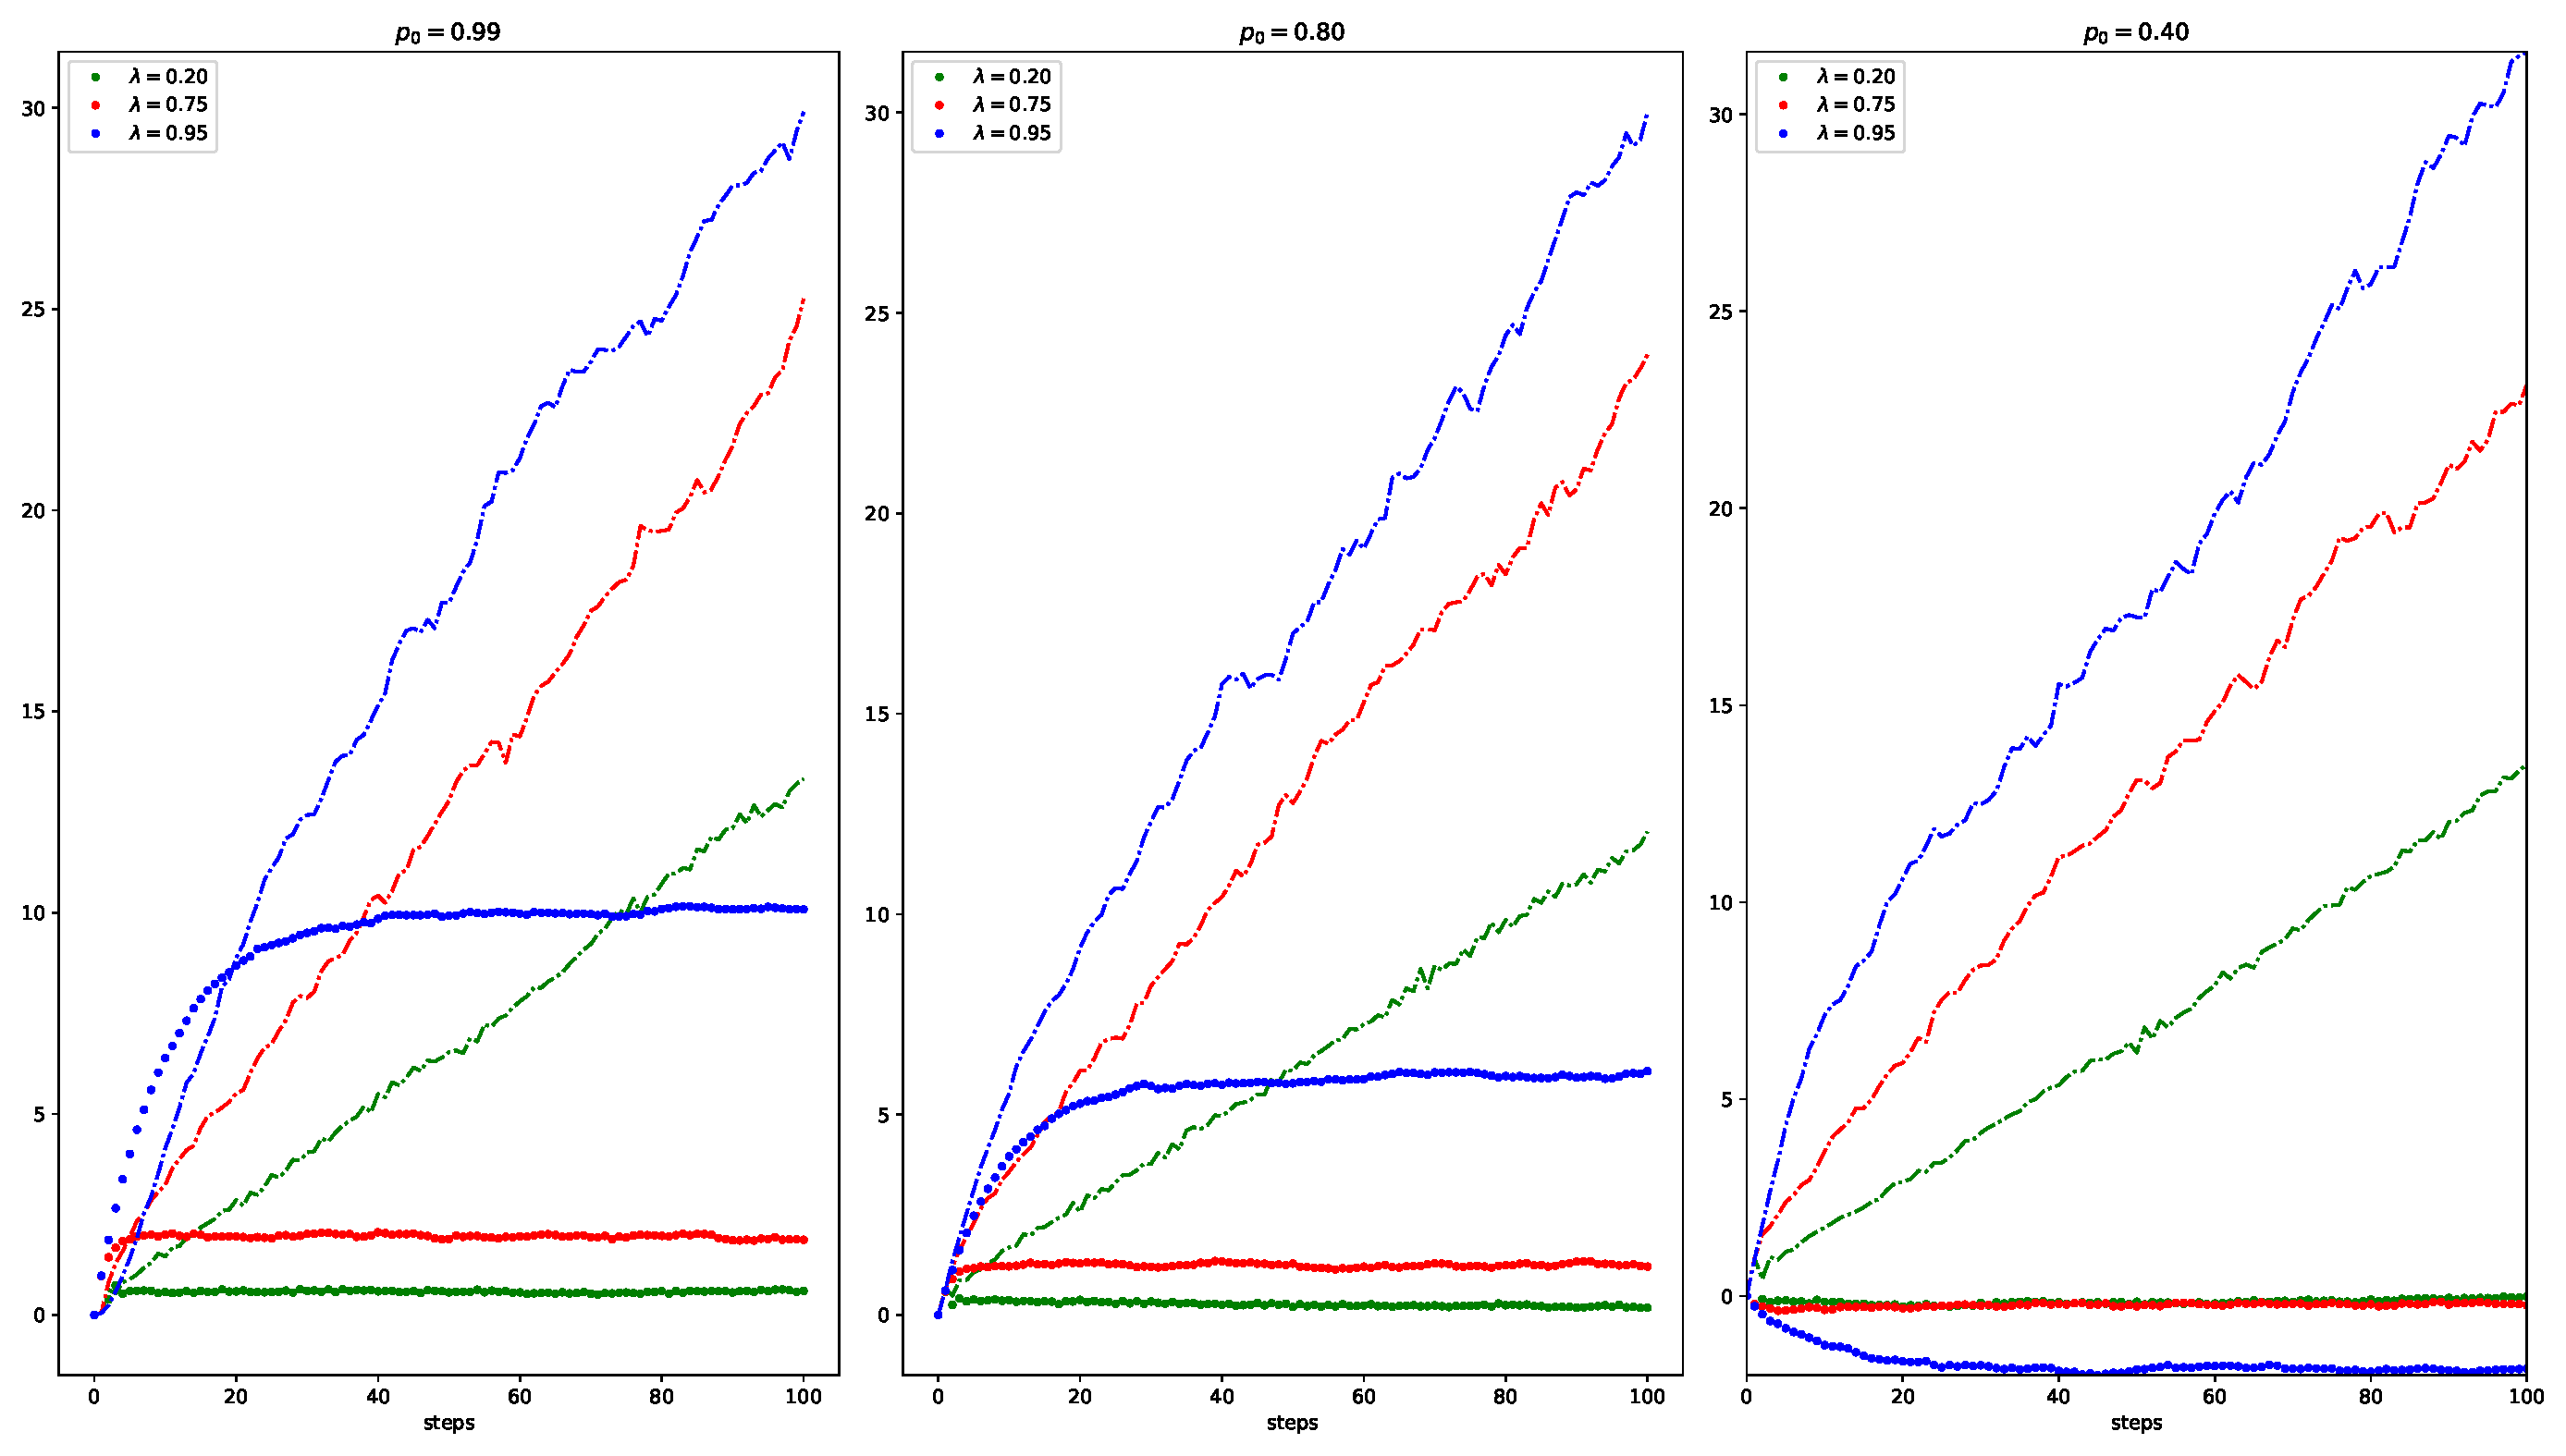
\includegraphics[width=1\textwidth]{../simulations/e_position_1000_walks_100_steps_type_success_punished}
\centerline{\epsfbox{am335-2_1.eps}}
\caption{The observed average position of the walker (dotted, ``thicker'') of a \emph{success punishing} version of the random walk and its variance (dashed lines, ``thinner''). The values were computed from 1000 simulated realizations of each parameter combination.}\label{fig:position-punished}
\bigskip

\section{Random walk with varying transition probability---alternatives}\label{sec:Random-walk-aternatives}

\subsection{Success rewarding model}\label{subsec:success-rewarding-model}
The basic definition of the random walk (Defi\-nition~\ref{success_punished})
presents a \emph{success punishing} model, meaning that the probability
of an event is decreased every time that event occurs.
The opposite situation
can be considered, where the probability of an event is increased
with each event's occurrence.
Formally, such a random walk is defined
in a following manner~\cite{ja2019teze}:

\begin{definition}
\label{succes_rewarded}Let ${\{X_{n}\}}_{n=1}^{\infty}$, $p_{0}$
and $\lambda$ be as in Definition~\ref{success_punished}.
Further
let ${\{P_{n}\}}_{n=1}^{\infty}$ be a sequence of discrete random
variables given by
\begin{eqnarray}
P_{1}=&\lambda p_{0}+\frac{1}{2}(1-\lambda)(1+X_{1}),\label{eq:P1_def-reward}
\\
P_{i}=&\lambda P_{i-1}+\frac{1}{2}(1-\lambda)(1+X_{i})\quad\forall\, i\geq2.\label{eq:Pi_def-reward}
\end{eqnarray}

The sequence ${\{S_{n}\}}{}_{n=0}^{\infty},$ given as in Definition~\ref{success_punished}, is a random walk with varying probabilities---\emph{success rewarding}.
\end{definition}

In this section, all variables ($P,X,S$) are related to the
\emph{success rewarding} model.
This version of the model behaves differently
than the \emph{success punishing} version, which can be observed with
the help of the following propositions.

\begin{proposition}
For all $t\ge 2,$
\begin{equation}
P_{t}=p_{0}\lambda^{t}+\frac{1}{2}(1-\lambda)\sum_{i=1}^{t}\lambda^{t-i}(1+X_{i}).\label{eq:propSuccess1}
\end{equation}
\end{proposition}

\begin{proof}
The Proposition is proved using mathematical induction.
For $t=2$ using (\ref{eq:P1_def-reward})
and (\ref{eq:Pi_def-reward}), we find that
$$
\aligned
P_{2}=\lambda P_{1}+\frac{1}{2}(1-\lambda)(1+X_{2})&=\lambda\Big(\lambda p_{0}+\frac{1}{2}(1-\lambda)(1+X_{1})\Big)+\frac{1}{2}(1-\lambda)(1+X_{2})\\
&=p_{0}\lambda^{2}+\frac{1}{2}(1-\lambda)\sum_{i=1}^{2}\lambda^{2-i}(1+X_{i})
\endaligned
$$
which is in accordance with~\eqref{eq:propSuccess1}.
Now, for the
induction step $t\rightarrow t+1$ we obtain from (\ref{eq:Pi_def-reward})
and the induction assumption
$$
\aligned
P_{t+1}&=\lambda P_{t}+\frac{1}{2}(1-\lambda)(1+X_{t+1})\\
&=\lambda\bigg(p_{0}\lambda^{t}+\frac{1}{2}(1-\lambda)\sum_{i=1}^{t}\lambda^{t-i}(1+X_{i})\bigg)+\frac{1}{2}(1-\lambda)(1+X_{t+1})\\
&=p_{0}\lambda^{t+1}+\frac{1}{2}(1-\lambda)\sum_{i=1}^{t}\lambda^{t-i+1}(1+X_{i})+\frac{1}{2}(1-\lambda)(1+X_{t+1})\\
&=p_{0}\lambda^{t+1}+\frac{1}{2}(1-\lambda)\sum_{i=1}^{t+1}\lambda^{t+1-i}(1+X_{i}).
\endaligned
$$
\end{proof}

\begin{proposition}
\label{PropReward2}For all $t\geq1,$ $E(P_{t})=p_{0}.$
\end{proposition}

\begin{proof}
Using $E(X_{t}|P_{t-1})=2P_{t-1}-1$ and (\ref{eq:Pi_def-reward}),
we obtain
$$
\aligned
EP_{t}=E[E(P_{t}|P_{t-1})]=&E\Big[E(\lambda P_{t-1}+\frac{1}{2}(1-\lambda)(1+X_{t})|P_{t-1})\Big]\\
=&E\Big[\lambda P_{t-1}+\frac{1}{2}(1-\lambda)(1+2P_{t-1}-1)\Big]\\
=&E[\lambda P_{t-1}+(1-\lambda)P_{t-1})=E(P_{t-1}).
\endaligned
$$
Recursively we get
\begin{equation}
E(P_{t})=E(p_{0})=p_{0}.\label{eq:EPt-reward-formula}
\end{equation}
\end{proof}

\begin{proposition}
The sequence $X_t$ is a stationary sequence of Bernoulli random
variables with values $1,-1$ and with $P(X_t=1)=p_0$.
\end{proposition}

\begin{proof}
As the distribution of $X_t$ is fully given by $E(P_{t-1})$, the
statement follows directly from Proposition~\ref{PropReward2}.
\end{proof}

Further, we can calculate the expected position of the walker at a given step $t$ just from the knowledge of the input parameters.

\begin{proposition}
For all $t\geq1,$
\[
E(S_{t})=S_{0}+t(2p_{0}-1).
\]
\end{proposition}


\begin{proof}
As $EX_{t+1}=E[E(X_{t+1}|P_t)]=E(2P_t -1)$, using the result of Proposition~\ref{PropReward2}, we get
\[
E(S_{t+1})= {E(S_{t}+X_{t+1}) = ES_{t}+E(2P_{t}-1)}=
ES_{t}+(2p_{0}-1)
\]

which then recursively proves the statement.
\end{proof}

\begin{corollary}
For $t\rightarrow\infty,$
\[
\lim_{t\to\infty}E(S_{t})=\begin{cases}
   \infty & p_{0}>\frac{1}{2},\\
   0 & p_{0}=\frac{1}{2},\\
   -\infty & p_{0}<\frac{1}{2}.
\end{cases}
\]
\end{corollary}

\begin{proposition}
For all $t\geq1,$
\begin{equation}
\Var(P_{t})=(2\lambda-\lambda^{2})^{t}p_{0}^{2}+p_{0}(1-\lambda)^{2}\sum_{i=1}^{t}(2\lambda-\lambda^{2})^{t-i}-p_{0}^{2}.\label{eq:VarPt-reward-prop}
\end{equation}
\end{proposition}

\begin{proof}
The proof will be done in several steps, similarly to the proof of Proposition~\ref{PropVarP-succes}.
It is based on the definition of variance~\eqref{eq:VarP-definition}.
{}From Proposition~\ref{PropReward2} it\vadjust{\goodbreak} follows $E(P_{t})=p_{0}$ that and
it is thus sufficient to prove that
\begin{equation}
E(P_{t}^{2})=(2\lambda-\lambda^{2})^{t}p_{0}^{2}+p_{0}(1-\lambda)^{2}\sum_{i=1}^{t}(2\lambda-\lambda^{2})^{t-i}.\label{eq:Ept2-finalvzorec-reward}
\end{equation}
The proof will be done using mathematical induction again.
First observe that
\begin{equation}
\topaligned
E(P_{t}^{2})&=E[E(P_{t}^{2}|P_{t-1})]=E\Big[E\Big(\lambda P_{t-1}+\frac{1}{2}(1-\lambda)(1+X_{t})\Big)^{2}|P_{t-1}\Big]
\\
  &  =EP_{t-1}^{2}(2\lambda-\lambda^{2})+p_{0}(1-\lambda)^{2},\label{eq:EPt-EPt-1-reward}
  \endaligned
\end{equation}
where the facts that $E[(1+X_{t})^{2}|P_{t-1}]=4P_{t-1}$, $E[(1+X_{t})|P_{t-1}]=2P_{t-1}$
and Proposition~\ref{PropReward2} were used.
Now for $t=1$ we get
\[
EP_{1}^2=p_{0}^{2}(2\lambda-\lambda^{2})+p_{0}(1-\lambda)^{2}=(2\lambda-\lambda^{2})^{1}p_{0}^{2}+p_{0}(1-\lambda)^{2}\sum_{i=1}^{1}(2\lambda-\lambda^{2})^{1-i}
\]
and thus~\eqref{eq:Ept2-finalvzorec-reward} holds for $t=1$.
For the induction step $t\rightarrow t+1$
we get from the induction assumption and (\ref{eq:EPt-EPt-1-reward})
   $$
  \aligned
E(P_{t+1}^{2})&=EP_{t}^{2}(2\lambda-\lambda^{2})+p_{0}(1-\lambda)^{2}\\
&=((2\lambda-\lambda^{2})^{t}p_{0}^{2}+p_{0}(1-\lambda)^{2}\sum_{i=1}^{t}(2\lambda-\lambda^{2})^{t-i})\cdot(2\lambda-\lambda^{2})+p_{0}(1-\lambda)^{2}\\
&=(2\lambda-\lambda^{2})^{t+1}p_{0}^{2}+p_{0}(1-\lambda)^{2}\sum_{i=1}^{t}(2\lambda-\lambda^{2})^{t-i+1}+p_{0}(1-\lambda)^{2}\\
&=(2\lambda-\lambda^{2})^{t+1}p_{0}^{2}+p_{0}(1-\lambda)^{2}\sum_{i=1}^{t+1}(2\lambda-\lambda^{2})^{t+1-i}.
\endaligned
$$
The Proposition is then proved by substituting (\ref{eq:EPt-reward-formula})
and (\ref{eq:Ept2-finalvzorec-reward}) into~\eqref{eq:VarP-definition}.
\end{proof}


Notice that the last sum in (\ref{eq:VarPt-reward-prop}), after re-indexing
by $j=t-i$, yields
\[
\sum_{j=0}^{t-1}(2\lambda-\lambda^{2})^{j}=\frac{1-(2\lambda-\lambda^{2})^{t}}{1-2\lambda+\lambda^{2}}.
\]
Hence, the limit follows immediately:

\begin{corollary}
For $t\rightarrow\infty,$
\[
\lim_{t\to\infty}\Var(P_{t})=p_{0}(1-p_{0}).
\]
\end{corollary}

\begin{proposition}
For all $t\geq1$ we have
\[
\Var(X_{t})=4p_0(1-p_0).
\]
\end{proposition}

\begin{proof}
As $E(X_t)=2p_0-1$ and $E(X_t^2)=1$ the proof follows similarly as in Proposition~\ref{propVarX} directly from the definition of variance.
\end{proof}

\subsection{Two-parameter models}\label{subsec:two-parameter-models}
Another level of complexity can be added by using separate $\lambda$
parameters for each direction of the walk.
Again, two ways of handling
success are available.

\begin{definition}
\label{2lambdas} Let ${\{X_{n}\}}_{n=1}^{\infty}$ and $p_{0}$ be
as in Definition~\ref{success_punished}.
Further, let $\lambda_{0},\lambda_{1}\in(0,1)$
be constant coefficients and ${\{P_{n}\}}_{n=1}^{\infty}$ be a sequence
of discrete random variables given by
\begin{eqnarray}
P_{1}&=\frac{1}{2}[(1+X_{1})\lambda_{0}p_{0}+(1-X_{1})(1-\lambda_{1}(1-p_{0}))],\label{eq:P!1_def-1-1}
\\
P_{i}&=\frac{1}{2}[(1+X_{i})\lambda_{0}P_{i-1}+(1-X_{i})(1-\lambda_{1}(1-P_{i-1}))]\quad \forall\, i\geq2.\label{eq:Pi_def-1-1}
\end{eqnarray}
The sequence ${\{S_{n}\}}{}_{n=0}^{\infty},$ given as in Definition~\ref{success_punished}, is a random walk with varying probabilities---\emph{two-parameter success
punishing}.
\end{definition}


\begin{definition}
\label{2lambdas-reward}Let ${\{X_{n}\}}_{n=1}^{\infty}$ and $p_{0}$
be as in Definition~\ref{success_punished}, $\lambda_{0}$,$\lambda_{1}$
as in Definition~\ref{2lambdas} and ${\{P_{n}\}}_{n=1}^{\infty}$ be a sequence
of discrete random variables given by
$$
\aligned
P_{1}&=\frac{1}{2}[(1-X_{1})\lambda_{0}p_{0}+(1+X_{1})(1-\lambda_{1}(1-p_{0}))],\\
P_{i}&=\frac{1}{2}[(1-X_{i})\lambda_{0}P_{i-1}+(1+X_{i})(1-\lambda_{1}(1-P_{i-1}))]\quad \forall\, i\geq2.
\endaligned
$$
The sequence ${\{S_{n}\}}{}_{n=0}^{\infty},$ given as in Definition~\ref{success_punished}, is a random walk with varying probabilities---\emph{two-parameter success
rewarding}.
\end{definition}

Derivation of model properties is not so straightforward.
The development
of transition probability and its variance for different starting
probabilities $p_{0}$ and memory coefficient pairs $ [\lambda_{0},\lambda_{1}]=\bar{\lambda}$
for the \emph{two-parameter success punishing} version of the model
is shown in Figure~\ref{fig:Development-punish2l}.
Similarly as in
the single $\lambda$ version of the model, the variance seems to
depend on the $\bar{\lambda}$ pair only.
The expected transition
probability seems to converge to a constant value independently on
both the starting probability~$p_{0}$ and the memory coefficients $\bar{\lambda}$.
This interesting property of the walk will be the subject of a further study.

\midinsert
\centerline{\epsfbox{am335-3_1.eps}}
\caption{The development of the observed average
transition probability (dotted, upper part of the figure) of a \emph{two-parameter success
punishing} version of the random walk and its variance (dashed lines, lower part of the figure).
The values
were computed from 1000 simulated realizations of each parameter
combination.}\label{fig:Development-punish2l}
\endinsert

\subsection{Other alternatives}\label{subsec:other-alternatives}
The presented model of a random walk can be further developed and
more versions can be derived and described.
These variants include,
but are not limited to, a multidimensional walk (with either one or multiple
$\lambda$ parameters, \emph{success rewarding} or \emph{success
punishing}), a walk with the transition probability explicitly dependent
on more than the last step, i.e.~$P_{t}(k)\sim P_{t}(X_{t}, X_{t-1},\dots,X_{t-(k-1)})$,
or a walk with $\lambda$ parameter not constant, but a function
of the time~$t$, i.e.~$P_{t}(\lambda(t)$).
Detailed properties of
such walks together with their possible applications to real life
problems will be the subject of a further study.


\section{Simulations}\label{sec:Simulations}

A simulation study was performed in order to verify the possible usage of the
presented model in real life situations, namely on multiple processes
with relatively few events
(i.e.~multiple short walks of the same kind).
Such processes include for example the recurrence of diseases (few recurrences
but many patients), reliability of machines (few failures but multiple same machines)
or the modelling of sports (few significant events in a match but multiple matches).
The experiment consisted of generating $K$ random walks of length~$n$,\vadjust{\goodbreak}
of the same walk type and parameter configuration, and estimating the walk type and parameter values from the generated data.
Four different tasks were considered:
\begin{itemize}
\item[(1)] find $\lambda$ or $[\lambda_{0},\,\lambda_{1}]$ (further denoted as $\tilde{\lambda}$) with known $p_{0}$ and model type,
\item[(2)] find $p_{0}$ with known $\tilde{\lambda}$ and model type,
\item[(3)] find $p_{0}$ and $\tilde{\lambda}$ with known model type,
\item[(4)] find model type without any prior knowledge.
\end{itemize}
\bgroup\let\,\relax
The following parameter values were considered for data generation: $K\in\{5,\,100\}$, $n\in\{5,\,10,\,50,\,100\}$, $p_{0}\in\{0.5,\,0.8,\,0.9,\,0.99\}$, $\lambda\in\{0.5,\,0.8,\,0.9,\,0.99\}$ and $[\lambda_{0},\,\lambda_{1}]\in\{[0.5,\,0.8],\,[0.1,\,0.5],\,[0.5,\,0.99],\,[0.99,\,0.9]\}$.\egroup


Tasks 1--3 were solved using the maximum likelihood estimate (MLE), see~\cite{rossi2018mathematical}.
The derivation of the theoretical likelihood values is rather complicated; therefore a~numerical approach using the Python programming language and its scientific package SciPy was applied.
The Akaike Information Criterion ${\rm AIC}=2k-2\ln(\hat{L})$, where $k$ is the number of model parameters and $\hat{L}$ is the maximal likelihood, was then used for the last task.

Each experiment was repeated independently $N=100$ times for each parameter combination and sample characteristics were computed from the $100$ parameter estimates.
To assess the quality of the parameter estimation (tasks~1--3), four different evaluation criteria were tested.
\begin{itemize}
\item[(1)] the true parameter value lies within the standard $(1-\alpha)$ two-sided confidence interval around the mean,
\item[(2)] the true parameter value lies within the ``percentile'' interval, i.e.~between the $100\frac{{\alpha}}{2}$th and $100(1-\frac{1}{2}\alpha)$th percentile,
\item[(3)] the mean fitted parameter value lies within the ``proximity'' interval around the true parameter value $\omega$, computed as $[\omega-\frac{1}{2}\alpha\omega,\omega+\frac{1}{2}\alpha\omega]$,
\item[(4)] the median fitted parameter value lies within the ``proximity'' interval.
\end{itemize}

To evaluate task~4, all four presented models were fitted on the set of $K$ walks and the AIC was computed for each one of them.
The model with the lowest AIC value was then selected.
The quality of such estimation for the given walk configuration was then assessed using the proportion of the number of correctly chosen models to the number of analyzed walk sets $N$.

The above mentioned criteria serve only as an approximate tool to evaluate the estimate's quality, however the results show that the model can be successfully fitted to empirical data.
For $K=100$, $\alpha=0.1$ and all combinations of input parameters and walk lengths $\tilde{\lambda}$, $p_0$ and $n$, $92\%$ of all evaluation criteria (for tasks~1--3) were successful and the correct model was found in $85\%$ of cases (task~4).
As expected, the results are less convincing for $K=5$, with only $73\%$ of all evaluation criteria being successful and $70\%$ of correctly found models.
An example of the parameter estimation evaluation can be seen in Table~\ref{tab:Fitting-results} (there just task~1), and an example of the model type identification results (task~4) can be observed in Table~\ref{tab:Fitting-results-model}.
Both tables contain only a brief illustration of results due to space limitations.
Full results of all evaluation setups, i.e.~combinations of input parameters $\tilde{\lambda}$ and $p_0$, number of observed walks $K$ and their different lengths $n$ as well as several values of parameter $\alpha$ can be found in the GitHub repository (see the last paragraph of the paper).

\midinsert
\setbox0\vbox{\let\\=\cr
\halign{\hss#\hss \vrule width0pt height10pt depth4pt
&&\quad\hss\strut#\unskip\hss\cr\hline
&&  Type & mean &  st.\ dev. &  median &  percentile \\
\hline
 {$K=100$} &
{$n=5$}
& SP & 0.505 & 0.043 & 0.504 & $[0.439,0.576]$ \\
& & SR & 0.502 & 0.033 & 0.503 & $[0.451,0.549]$ \\
& & SP2 & 0.505 & 0.060 & 0.501 & $[0.399,0.606]$ \\
& & SR2 & 0.491 & 0.047 & 0.490 & $[0.415,0.564]$ \\
%\hline
&{$n=100$}
& SP & 0.499 & 0.008 & 0.499 & $[0.484,0.511]$ \\
& & SR & 0.502 & 0.022 & 0.502 & $[0.460,0.535]$ \\
& & SP2 & 0.502 & 0.012 & 0.502 & $[0.478,0.521]$ \\
& & SR2 & 0.498 & 0.026 & 0.501 & $[0.452,0.535]$ \\
\hline
{$K=5$}&
{$n=5$}&
 SP & 0.468 & 0.155 & 0.495 & $[0.214,0.690]$ \\
& & SR & 0.489 & 0.214 & 0.499 & $[0.000,0.830]$ \\
& & SP2 & 0.462 & 0.209 & 0.464 & $[0.139,0.780]$ \\
& & SR2 & 0.521 & 0.211 & 0.527 & $[0.123,0.923]$ \\
%\hline
&{$n=100$}&
 SP & 0.493 & 0.037 & 0.494 & $[0.419,0.554]$ \\
& & SR & 0.485 & 0.102 & 0.496 & $[0.391,0.624]$ \\
& & SP2 & 0.497 & 0.056 & 0.498 & $[0.405,0.586]$ \\
& & SR2 & 0.461 & 0.173 & 0.513 & $[0.001,0.655]$\\
\hline
}}
\centerline{\box0}
\figure
Table~1. The table shows an example of task $1$ evaluation results,
with true parameter values $\lambda=0.5$ or $\lambda_{0}=0.5$ (and corresponding $\lambda_{1}=0.8$), and $p_0=0.5$, $\alpha=0.1$.
The mean of parameter estimates and its standard deviation and the median of parameter estimates and the corresponding ``percentile'' interval are presented.
\emph{SP} stands for \emph{success punishing}, \emph{SR} for \emph{success rewarding}, the number $2$ denotes the model with two $\lambda$ parameters.\label{tab:Fitting-results}


\setbox0\vbox{\let\\=\cr
\halign{\hss#\hss \vrule width0pt height10pt depth4pt
&&\quad\hss#\unskip\hss\cr\hline
K &  $n$ & SP &  SR &  SP2 &  SR2
  \\
\hline
{$100$}
& 5 & 83\% & 80\% & 100\% & 100\% \\
& 100 & 86\% & 88\% & 100\% & 100\% \\
\midrule
{$5$}
& 5 & 84\% & 85\% & 42\% & 34\% \\
& 100 & 82\%  & 80\% & 100\% & 93\% \\
  \hline
  }}
\bigskip
\centerline{\box0}
\figure Table~2.
The table shows model estimation success rate.
Notation and parameter configuration is the same as in Table~\ref{tab:Fitting-results}. \label{tab:Fitting-results-model}

\hrule height0pt
\endinsert
% \bigskip

Longer walks show generally better results when finding the coefficients $\tilde{\lambda}$ especially for the \emph{success rewarding} version of the model (as seen for example in row 10 in Table~\ref{tab:Fitting-results}), while the performance of finding correct $p_0$ seems independent on the walk's length.
This is not surprising, as the parameter $p_0$ affects mostly the first few steps of the walk, while $\tilde{\lambda}$ play their role thorough the entire course of the walk.
As expected, tasks~1--2 show better results than task~3, as there are less parameters to estimate.



\section{Conclusion}\label{sec:Conclusion}

This work follows up on the recent results on random walks with varying
probabilities.
It describes and proves certain properties of such
a walk, while other properties have been studied with the help of numerical
methods.
The study also shows the results of the maximum likelihood
and AIC based estimations of model parameters and types using optimization
procedures.
The method has been successfully tested on a~set of randomly
generated data.
The presented model has also many possible uses in
real life applications.
Such a type of random walk describes especially
well processes where either a single or just a small number of events
can significantly affect the future development of the process.
Such
processes can be found in reliability analysis, medical as well as
econometric studies, and very often in sports modeling.
The authors recently presented a study where the \emph{success rewarding} model was applied
to predict the \emph{in-play} development of a Grand Slam tennis matches
with compelling results when used for live betting against a bookmaker~\cite{ja2019mathsport_proc}.

The source code containing all functionality mentioned in this article
is freely available as open source at
GitHub ({\tt https://github.com/tomaskourim/amistat2019}).



\Refs

%\bibitem{davis2012theory}
\no 1
\by R.\,A.\,Davis, H.\,Liu
\paper Theory and inference for a class of nonlinear models with application to time series of counts
\jour Stat. Sin.
\vol 26 \yr 2016 \pages 1673--1707
\ZBL 1356.62137
\MR 3586234
\DOI 10.5705/ss.2014.145t

%\bibitem{feller1957introduction}
\no 2
\by W.\,Feller
\book An Introduction to Probability Theory and Its Applications
\publ A Wiley Publication in Mathematical Statistics. John Wiley \& Sons, New York \yr 1957
\ZBL 0077.12201
\MR 0088081

%\bibitem{hawkes1971spectra}
\no 3
\by A.\,G.\,Hawkes
\paper Spectra of some self-exciting and mutually exciting point processes
\jour Biometrika
\vol 58 \yr 1971 \pages 83--90
\ZBL 0219.60029
\MR 0278410
\DOI 10.1093/biomet/58.1.83

%\bibitem{ja2017ddny}
\no 4
\by T.\,Kou\v rim
\paper Random walks with varying transition probabilities
\inbook Doktorandsk\'e dny 2017
\publ \v CVUT, FJFI, Praha \yr 2017
\eds P.\,Ambro\v z, Z.\,Mas\'akov\'a

%\bibitem{ja2019mathsport_proc}
\no 5
\by T.\,Kou\v rim
\paper Random walks with memory applied to grand slam tennis matches modeling
\inbook MathSport International 2019: Conference Proceedings
\publ Propobos Publications, Athens \yr 2019
\pages 220--227

%\bibitem{ja2019teze}
\no 6
\by T.\,Kou\v rim
\book Statistical Analysis, Modeling and Applications of Random Processes with Memory: PhD Thesis Study
\publ \v CVUT FJFI, Praha \yr 2019

%\bibitem{ja2019imam}
%\no 7
%\by T.\,Kou\v rim, P.\,Volf
%\paper Tennis match as random walk with memory: Application to %Grand slam matches modelling
%\jour Submitted to IMA Journal of Management Mathematics \yr 2019

%\bibitem{pearson1905problem}
\no 7
\by K.\,Pearson
\paper The problem of the random walk
\jour Nature
\vol 72 \yr 1905 \pages 342
\JFM 36.0303.02
\DOI 10.1038/072342a0

%\bibitem{rossi2018mathematical}
\no 8
\by R.\,J.\,Rossi
\book Mathematical Statistics: An Introduction to Likelihood Based Inference
\publ John Wiley \& Sons, Hoboken \yr 2018
\ZBL 1407.62006
\DOI 10.1002/9781118771075

%\bibitem{schutz2004elephants}
\no 9
\by G.\,M.\,Sch\"utz, S.\,Trimper
\paper Elephants can always remember: Exact long-range memory effects in a non-Markovian random walk
\jour Phys. Rev. E
\vol 70 \yr 2004 \pages Article ID 045101
\DOI 10.1103/PhysRevE.70.045101

%bibitem{turban2010random}
\no 10
\by L.\,Turban
\paper On a random walk with memory and its relation with Markovian processes
\jour J. Phys. A, Math. Theor.
\vol 43 \yr 2010 \pages Article ID 285006, 9 pages
\ZBL 1204.82022
\MR 2658904
\DOI 10.1088/1751-8113/43/28/285006


\adresy
{\it Tom\'a\v{s} Kou\v rim}, Faculty of Nuclear Sciences and Physical Engineering, Czech Technical University in Prague,
B\v rehov\'a 7, 115\,19 Praha 1,
Czech Republic,
e-mail: {\tt kourim@outlook.com};
{\em Petr Volf}, Institute of Information Theory and Automation, Academy of Sciences of the Czech Republic,
Pod Vod\'arenskou v\v e\v z\'{\i} 4, 182\,00 Praha 8,
Czech Republic,
e-mail: {\tt volf@utia.cas.cz}



\bye
